\section{優美動作の評価}

\subsection{従来手法}
上田研ではこれまで多くのモデルが提唱されてきた.
その多くは稲津\cite{inazu2}の全曲率計算を起源としている.
先に挙げたB-spline近似で手先軌道を曲線近似し,図\ref{curves}のように
全曲率$\mu$が0.87~1.31となる曲線を多く含むものを優美としている.
そこから面積や角度に派生するモデルも存在するが,根底は手先軌道である.
今回作成したネットワークが「優美」と判定したものは動画のどの箇所を根拠に
「優美」と判断したのか,動作を抽出して検証する際,どこに着目すべきと
示唆しているかなどを検証した.

\begin{figure}[b]
  \begin{center}
    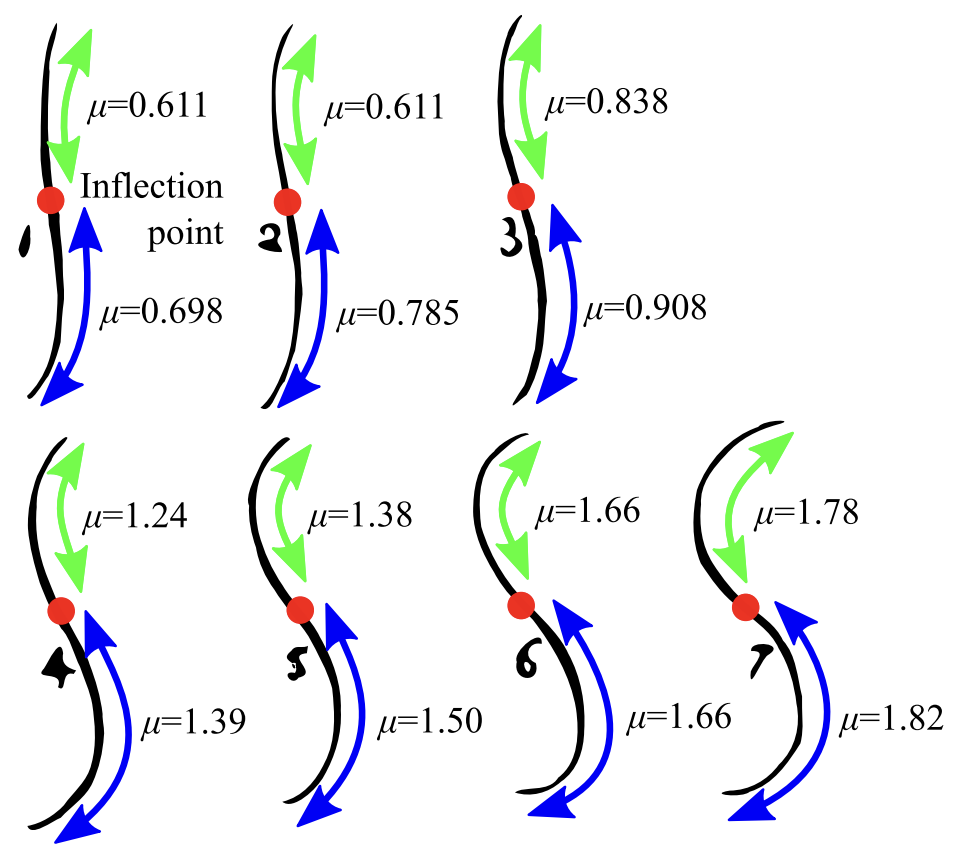
\includegraphics[width=100mm]{images/quote/curves.png}
  \end{center}
  \caption{Hogarth Curveの全曲率}
  \label{curves}
\end{figure}

\subsection{Grad Camを用いた評価}
作成したネットワークの判断根拠を可視化するために,Pytorch-GradCam\cite{pygradcam}を
使用した.作成したネットワークはPytorch\cite{pytorch}でできているので,GradCamも
同じくPytorchでできたものを使用した.

\subsection{確率分布を用いた評価}

\subsection{従来手法との比較}